\documentclass[]{article}
\usepackage[margin = 1.5in]{geometry}
\setlength{\parindent}{0in}
\usepackage{amsmath}
\usepackage{amsfonts}
\usepackage{amssymb}
\usepackage{amsthm}
\usepackage{pgfplots}
\usepackage[lined]{algorithm2e}
\usepackage{hyperref}
\usepackage[T1]{fontenc}
\usepackage{ae,aecompl}

\theoremstyle{definition}
\newtheorem{defn}{Definition}[section]
\newtheorem{ex}{Example}[section]

\setlength{\marginparwidth}{1.5in}
\setlength{\algomargin}{0.75em}
\newcommand{\lecture}[1]{\marginpar{{\footnotesize $\leftarrow$ \underline{#1}}}}

\begin{document}

	\title{\bf{CS 240: Data Structures and Data Management}}
	\date{Winter 2013, University of Waterloo \\ \center Notes written from Alejandro L\'opez-Ortiz's lectures.}
	\author{Chris Thomson}
	\maketitle
	\newpage

	\section{Introduction \& Code Optimization} \lecture{January 8, 2013}
		\subsection{Course Structure}
			The grading scheme is 50\% final, 25\% midterm, and 25\% assignments. There are five assignments, usually due on Wednesday mornings at 9:30 am. There are several textbooks for the course, all of which are optional but recommended. The textbooks cover roughly 80\% of the course content. There are also some course notes published online from previous terms, however the lectures will not necessarily follow those notes strictly.
			\\ \\
			See the \href{https://www.student.cs.uwaterloo.ca/~cs240/w13/info.phtml}{course syllabus} for more information.
			
		\subsection{CS as the Science of Information}
			So far in our undergraduate careers, computer science has meant programming. However, programming is only a subset of computer science. Computer science is the \textbf{science of information}.
			\\ \\
			What do we want to do with information? We want to:
			\begin{itemize}
				\item \textbf{Process it}. Programs $\equiv$ algorithms.
				\item \textbf{Store it}. We want to encode it. This also leads to information theory. Storing information involves data structures, databases, (file) systems, etc., all of which are searchable in some way.
				\item \textbf{Transmit it}. We want to transmit information over networks. This process involves coding theory.
				\item \textbf{Search it}. First, we have to structure it with data structures and/or SQL databases. Information retrieval is the process of searching for textual information instead of numerical information.
				\item \textbf{Mine it}. This involves artificial intelligence and machine learning.
				\item \textbf{Display it}. Information needs to be displayed using computer graphics (CG) and user interfaces (UI, partially related to psychology).
				\item \textbf{Secure it}. Encryption and cryptography are important. Information should also be stored redundantly to prevent harm from catastrophic events.
			\end{itemize}
	
		\subsection{Objectives of the Course}
			\begin{itemize}
				\begin{item}
					\textbf{Study efficient methods of storing, accessing, and performing operations on \underline{large} collections of data.} \\ \\
					``Large" is subjective -- your data needs to be large enough to justify the additional mental complexity. \\ \\
					Typical operations:
					\begin{itemize}
						\item Insert new item.
						\item ``Deleting" data (flagging data as ``deleted", not actually deleting the data).
						\item Searching for data.
						\item Sorting the data. \\
					\end{itemize}
				
					Examples of ``large data":
					\begin{itemize}
						\item The web.
						\item Facebook data.
						\item DNA data.
						\item LHC (Large Hadron Collider) measurements (terabytes per day).
						\item All the music from iTunes, for finding duplicate songs, etc.
					\end{itemize}
				\end{item}
				
				\begin{item}
					\textbf{There is a strong emphasis on mathematical analysis.} \\ \\
					The performance of algorithms will be analyzed using order notation.
				\end{item}
				
				\begin{item}
					\textbf{The course will involve abstract data types (objects) and data structures.} \\ \\
					We will see examples that have to do with:
					\begin{itemize}
						\item Databases.
						\item Geographic databases.
						\item Text searching.
						\item Text compression.
						\item Web searching.
					\end{itemize}
				\end{item}
			\end{itemize}
			
		\subsection{Code Optimization \& Measuring Performance}
			Richard Feynman was in charge of the computer group on the Manhattan Project. He made his code run 10x faster.
			\\ \\
			The initial method to measure performance was to use a \textbf{wall clock}. Initial studies looked like this:

			\begin{center}
				\begin{tabular}{|c|c|c|}
					\hline
					Data size & A & B \\ \hline
					3 & 1 & 3 \\
					5 & 2 & 9 \\
					10 & 4 & 10 \\
					20 & 16 & 11 \\ \hline
				\end{tabular}
			\end{center}
			
			However, computers were getting better, so we couldn't use wall clocks anymore. Results were not robust enough due to the qucik progression of performance increases in terms of computing power. Moreover, because of the differences in architecture, the same program may have a different execution time on two different computer models.
			\\ \\ 
			\underline{Idea}: rather than comparing algorithms using seconds, we should compare algorithms using the number of operations required for the algorithm to run.
			
			\begin{itemize}
				\item Express algorithm using pseudocode.
				\item Count the number of primitive operations.
				\item Plot the number of operations vs. the input size. \\
			\end{itemize}
			
			\begin{figure}
				\centering
				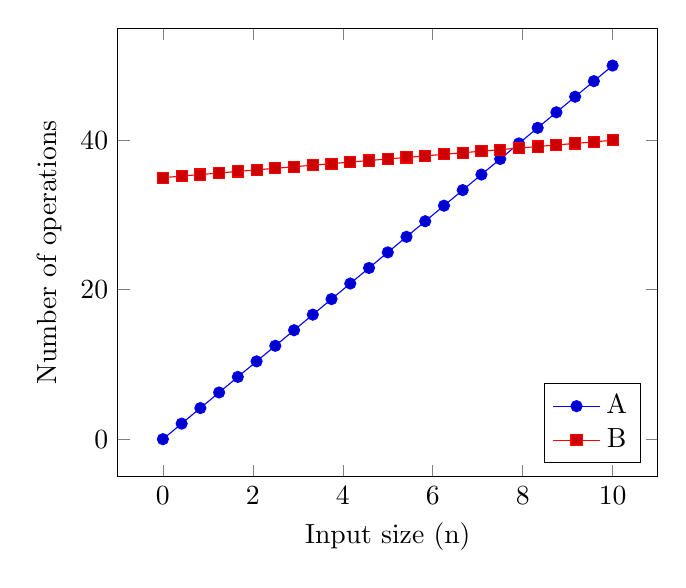
\begin{tikzpicture}[domain=0:10]
					\begin{axis}[
						xlabel = Input size (n),
						ylabel = Number of operations,
						legend entries = {A,B},
						legend pos = south east]
						\addplot{5*x};
						\addplot{0.5*x+35};
					\end{axis}
				\end{tikzpicture}
				\caption{A comparison of two algorithms $A$ and $B$.}
			\end{figure}
			
			Note that $A$ and $B$ are plotted as continuous functions, however they are not actually continuous -- we join all of the points for readability purposes only.
			\\ \\
			In the long run, you may want to use algorithm $B$ even if algorithm $A$ is better in some cases, because the benefits of $A$ will be short lived as $n$ grows.
			\\ \\
			Hence, comparing the programs has been transformed into comparing functions. We use order notation to measure the long-term growth of functions, allowing us to choose the smaller function, which corresponds to the faster algorithm.
	
	\section{Order Notation} \lecture{January 10, 2013}
		The time for algorithm $A$ on input of size $n$ is:
		
		\begin{align*}
			\underbrace{2n \log n}_\text{sort} + \underbrace{1.5n^3}_\text{mult} + \underbrace{22n^2 - 3n}_\text{additions} + \underbrace{7}_\text{setup}
		\end{align*}
		
		On a different machine, the same algorithm $A$ may be $2n \log n + 9n^3 + 10n^2 - 3n + 7$. These give a \textbf{false sense of precision}. These specifics can also be quite costly to determine. In the 1960s, Don Knuth proposed \textbf{order notation} as a way to analyze the general quality of algorithms in an accurate, cost- and time-efficient way by ignoring precise runtimes.
		
		\subsection{Formal Definitions}
			Order notation represents algorithms as functions. We say a function $f(n)$ relates to a certain order $g(n)$ using different notation depending on which relation we're interested in.
			\begin{center}
				\begin{tabular}{|c|c|}
					\hline
					 Relation & Functions \\ \hline
					 $3 \le 7$ & $f(n) = O(g(n))$ \\
					 $8 \ge 7$ & $f(n) = \Omega(g(n))$ \\
					 $7 = 7$ & $f(n) = \Theta(g(n))$ \\
					 $3 < 7$ & $f(n) = o(g(n))$ \\
					 $7 > 3$ & $f(n) = \omega(g(n))$ \\ \hline
				\end{tabular}
			\end{center}
			
			Here's an easy way to remember the correspondence between a relation and its order notation symbol: the greedy operators, $\le$ and $\ge$, are uppercase letters $O$ and $\Omega$. The less greedy operators, $<$ and $>$, are the same letters but in lowercase ($o$ and $\omega$). \\
			
			Order notation only cares about the long run. An algorithm can violate the relation early -- we're interested in its asymptotic behavior.
			
			\begin{defn}[$\le$]
				$f(n) = O(g(n))$ if there exist constants $c > 0, n_0 > 0$ such that $f(n) \le c \cdot g(n)$ for all $n \ge n_0$.
			\end{defn}
		
			\begin{defn}[$\ge$]
				$f(n) = \Omega(g(n))$ if there exist constants $c > 0, n_0 > 0$ such that $f(n) \ge c \cdot g(n)$ for all $n \ge n_0$.
			\end{defn}
			
			\begin{defn}[$=$]
				$f(n) = \Theta(g(n))$ if there exists constants $c_1, c_2 > 0$ such that $c_1 \cdot g(n) \le f(n) \le c_2 \cdot g(n)$.
			\end{defn}
			
			The equality relation is effectively sandwiching the algorithm $f(n)$ between two other functions (the squeeze theorem). If it's possible to sandwich the algorithm between two multiples of the same $g(n)$, then $f(x)$ is said to be equal to the order $g(n)$.
			
			\begin{defn}[$<$]
				$f(n) = o(g(n))$ if for all $c > 0$ there exists constant $n_0 > 0$ such that $f(n) < c \cdot g(n)$ for all $n \ge n_0$.
			\end{defn}
		
			\begin{defn}[$>$]
				$f(n) = \omega(g(n))$ if for all $c > 0$ there exists constant $n_0 > 0$ such that $f(n) > c \cdot g(n)$ for all $n \ge n_0$.
			\end{defn}
			
		\subsection{Order Notation Examples}
			\begin{ex}
				$2n^2 + 3n + 11 = O(n^2)$
				\\ \\
				We need to show that there exists constants $c > 0$ and $n_0 > 0$ such that $2n^2 + 3n + 11 \le cn^2$ for all $n \ge n_0$.
				\\ \\
				Let $c = 3$. Simplifying gets us $3n + 11 \le n^2$. This holds for $n_0 = 1000$, for instance.
			\end{ex}
			
			\begin{ex}
				$2n^2 + 3n + 11 1 = \Theta(n^2)$
				\\ \\
				In order to show equality ($\Theta$), we need to show both the $\le$ and $\ge$ cases. In the previous example, the $\le$ case was shown. For the $\ge$ case, we need to show $n^2 \le c \cdot (2n^2 + 3n + 11)$.
				\\ \\
				Let $c = 1$. Simplifying gets us $n^2 \le 2n^2 + 3n + 11$, which gives us $0 \le n^2 + 3n + 11$. This holds for $n_0 = 0$.
			\end{ex}
			
			\begin{ex}
				$2010n^2 + 1388 = o(n^3)$
				\\ \\
				We must show that for all $c > 0$, there exists $n_0 > 0$ such that $2010n^2 + 1388 \le c \cdot n^3$ for all $n \ge n_0$.
				
				\begin{align*}
					\frac{2010n^2+1388}{n^3} \stackrel{?}{\le} \frac{c \cdot n^3}{n^3} \implies \frac{2010}{n} + \frac{1388}{n^3} \stackrel{?}{\le} c
				\end{align*}
				
				There is a \textbf{trick to prove f(n) = o(g(n))}: show that $\lim_{n \to \infty}{}\frac{f(n)}{g(n)} = 0$.
			\end{ex}
		
		\subsection{A note about the use of =}
			\begin{align*}
				\underbrace{2n^2}_\text{specific function} \in \underbrace{O(n^2))}_\text{set of functions}
			\end{align*}
			
			The use of the equality operator ($=$) in order notation is not the same as in most other areas of mathematics, since a single element of a set cannot strictly be equal to the set itself (even $a \ne \{a\}$). The $=$ in order notation is not a true equality -- it's just notation. The $\in$ operator is semantically more correct.
		
		\subsection{Performance of Algorithms}
			We have made some progression in how we determine the performance of algorithms.
			\begin{itemize}
				\item Comparing single runs.
				\item Comparing measured curves (multiple runs).
				\item Produce analytical expressions for the curves.
				\item Simplify using order notation.
			\end{itemize}
			
			Let's say we have the problem of integrating a mathematical function. Our program numerically integrates the function, and we're trying to analyze the algorithm behind that process. The timing would vary depending on the mathematical function and precise required.
			\\ \\
			If we conduct multiple runs of our algorithm, we'll get different times. Plotting all of the results (time vs. input size) will result in data that is not a function, because the data fails the vertical line test, since for a given input size we have multiple times.
			\\ \\
			We need to decide on a convention for these cases where we have multiple time values. In this course, we'll usually look at the worst case, however in some situations examining the best or average cases could be useful.
			\\ \\
			Finding the average case is hard. To produce an appropriate average, we need an input distribution.
	\section{Formalism} \lecture{January 15, 2013}
		\begin{defn}
			A \textbf{problem} is a collection of questions and (correct) answer pairs.
		\end{defn}

		\begin{ex}
			Informally, the problem is ``multiplying two numbers.'' More formally, the problem could be represented as: (2 x 3, 6), (3 x 4, 12), (1 x 5, 5), etc.
		\end{ex}

		\begin{defn}
			An \textbf{instance} of a problem is a specific question and answer pair, (Q, A).
		\end{defn}

		\begin{defn}
			The \textbf{input} of a problem is the question. Example: 3 x 4.
		\end{defn}

		\begin{defn}
			The \textbf{output} is the only correct answer. Note: there is only one correct answer under this definition. ``Multiple'' correct answers can always be reduced to some canonical form that represents the one correct answer.
		\end{defn}

		\begin{defn}
			An \textbf{algorithm} is a mechanical method to produce the answer to a given question of a problem.
		\end{defn}
		
		\begin{defn}
			The \textbf{size of the input} is the number of bits, characters, or elements in the question. This definition will vary depending on what's most appropriate for the given question.
		\end{defn}

		Long division in elementary school was the first time a problem's complexity was directly related to the input size. That's not always the case, however.

		\begin{defn}
			We say an algorithm \textbf{solves} a problem if for every question $Q$ it produces the correct answer, $A$.
		\end{defn}

		\begin{defn}
			A \textbf{program} is an implementation of an algorithm using a specified computer language.
		\end{defn}

		\begin{ex}
			We want to sort $n$ numbers. One instance of this problem $Q$ is:
			\begin{align*}
				(\underbrace{(5, 1, 3, 2, 4)}_\text{Q}, \underbrace{(1, 2, 3, 4, 5)}_\text{A})
			\end{align*}

			For a problem in this form, we'll say the size of $Q$ is $|I| = 5$. Why? Counting the number of elements is the most logical definition in this case.
		\end{ex}

		This course emphasizes algorithms rather than programs. We're computer scientists, so we care about the algorithm and the speed/efficiency of that algorithm.
		\\ \\
		A problem $\Pi$ can have several correct algorithms that solve it. Our goal is to find efficient solutions to $\Pi$. How do we do that?
		\begin{enumerate}
			\item \textbf{Algorithm design}. Find a solution(s) to $\Pi$.
			\item \textbf{Algorithm analysis}. Assess the correctness and efficiency of the algorithm.
		\end{enumerate}

		In this course, we're mostly interested in algorithm analysis. Algorithm design will be covered in more detail in CS 341.

		\subsection{Timing Functions}
			A timing function is a function $T_{\mathcal{A}}$ such that:
			\begin{align*}
				T_{\mathcal{A}}: \{ Q \} \to \mathbb{R}^{+}
			\end{align*}
			where $\mathbb{R}^{+}$ is the set of positive real numbers.
			\\ \\
			$T_{\mathcal{A}}(Q)$ is the time taken by algorithm $\mathcal{A}$ to compute the answer to $Q$.
			\\ \\
			We also want to define a general timing function for a particular problem, regardless of algorithm: 
			\begin{align*}
				T(n) &= max \{T_{ \mathcal{A}}(Q) \} \\ 
				T_{avg}(n) &= avg \{ T_{\mathcal{A}}(Q) \} \\ 
				T_{min}(n) &= min \{ T_{\mathcal{A}}(Q) \} \\
				\vdots&
			\end{align*}

			If we had two solutions (algorithms) $T_A(n)$ and $T_B(n)$, we could use order notation to compare the quality of $A$ and $B$.
			\\ \\
			Note that some problem instances are easier than others to solve, even with the same input size. Most people find it easier to multiply $0 \times 7$ than $8 \times 7$, for instance, despite those two problems having the same input size.
	\section{Analysis of Algorithms}
		In order to analyze an algorithm, we count the number of \underline{basic} operations that the algorithm performs.
		\begin{ex}
			Let's say our algorithm is to compute $x^2 + 4x$ and assign it to a variable called \verb+result+. That involves seven basic operations:
			\begin{enumerate}
				\item Read $x$ from memory.
				\item Compute $x \cdot x$.
				\item Assign the result of $x \cdot x$ to a variable, \verb+pr1+.
				\item Compute $4 \cdot x$.
				\item Assign the result of $4 \cdot x$ to a variable, \verb+pr2+.
				\item Compute \verb+pr1+ + \verb+pr2+.
				\item Assign the result of \verb+pr1+ + \verb+pr2+ to a variable, \verb+result+.
			\end{enumerate}
		\end{ex}

		The number of operations remains the same across machines, but the actual running time of an algorithm will differ from machine to machine (which one of the reasons why we use order notation).
		\\ \\
		We only count the number of \underline{basic} operations. There are various definitions of what a ``basic'' operation actually is (especially with regards to variable assignments), but these are some common operations that are considered to be basic:
		\begin{itemize}
			\item Add numbers of reasonable size (numbers that can be added primitively).
			\item Multiply numbers of reasonable size (numbers that can multiplied primitively).
			\item Access an index in an array.
			\item Store a value in memory (variable assignments).
			\item Read a value from memory.	
		\end{itemize}
		Be careful. Some languages disguise complexity well. Just because the syntax is simple doesn't necessarily mean it's a basic operation, and doesn't guarantee that the operation runs in constant time.

		\subsection{Techniques for Algorithm Analysis}
			\begin{itemize}
				\item Straight line programs (no loops). Simply tally up the basic operation count.
				\item Loops (\verb+for+/\verb+while+). You need to add the number of operations for each pass on the body of the loop.
			\end{itemize}

			\begin{ex}
				Analyze the following algorithm. \\
				\begin{algorithm}[H]
					\For{i = a to b}{
						< straight line program > $T_L$
					}
				\end{algorithm}
				This program will run with $\sum_{i = a}^{b} T_L(i)$ operations.
			\end{ex}

			Whenever you have a loop in your algorithm, you should expect to get a summation in your timing function.
			\begin{ex}
				Analyze the following algorithm. \\
				\begin{algorithm}[H]
					\For{x = 0 to 10}{
						pr1 = x * x\;
						pr2 = 4 * x\;
						result = pr1 + pr2\;
						print result\;
					}
				\end{algorithm}

				This program will run with $\sum_{i = 0}^{10} 4 = 44$ operations (depending on your definition of ``basic'' operations).
			\end{ex}

			Operations like addition and multiplication are primitive for numbers of a reasonable size. Once numbers get large enough to exceed certain limits, we have to resort to some trickery to perform those operations, which adds additional complexity, making them no longer ``basic'' operations.
			\\ \\
			We can be a bit sloppy and use the worst case, then say the actual algorithm is $\le$ what we calculated.
			\begin{ex} 
				Analyze the following algorithm. Test 1 ($n$). \\
				\begin{algorithm}[H]
					sum = 0\;
					\For{i = 1 to n}{
						sum = sum + i
					}
					\Return sum
				\end{algorithm}
				This program will run with $1 + (\sum_{i = 1}^n 1) + 1 = 2 + n = \Theta(n)$ operations.
			\end{ex}

			\begin{ex}
				Analyze the following algorithm. \\
				\begin{algorithm}[H]
					sum = 0\;
					\For{i = 1 to n}{
						$sum = sum + (i - j)^2$\;
						$sum = sum^2$\;
					}
					\Return sum

				\end{algorithm}

				This program will run with time:
				\begin{align*}
					& 1 + \sum_{i = 1}^{n} \bigg[ \sum_{j = 1}^{i} 4 \bigg] + 1 \\
					&= 2 + \sum_{i = 1}^{n} 4i \\
					&= 2 + 4 \sum_{i = 1}^{n} i \\
					&= 2 + 4 \cdot \frac{n(n+1)}{2} \text{ (Gauss)} \\
					&= 2 + 2n^2 + 2n \\
					&= \Theta(n^2)
				\end{align*}

				We can be pessimistic, assume worst-case scenario, and say that it runs with time:
				\begin{align*}
					&2 + \sum_{i = 1}^{n} n \\
					&= O(n^2)
				\end{align*}

				Note that $O(n^2)$ is a less precise result than $\Theta(n^2)$, but in some cases that's good enough.
			\end{ex}

			Order notation helps make algorithm analysis easier by allowing us to throw away any specific constants, as long as the order remains untouched. The entire analysis process happens within the context of order notation, so you can just start dropping constants immediately.
			\\ \\
			Keep in mind, it is possible to create a bad over-estimation. You have to be smart about it.

			\begin{ex}
				Analyze the following algorithm. Test 2 (A, n). \\
				\begin{algorithm}[H]
					max = 0\;
					\For{i = 1 to n}{
						\For{j = 1 to n}{
							sum = 0\;
							\For{k = i to j}{
								sum = A[k] + sum\;
								\If{sum > max}{
									max = sum\;
								}
							}
						}
					}
					\Return max
				\end{algorithm}
				
				This is the \textbf{maximum subsequence problem}. The input is an array of integers $A[1\dots n]$, and the output is the consecutive run with the largest sum.
				\\ \\
				Sample sequence:
				\begin{tabular}{|c|c|c|c|c|c|c|}
					\hline 2 & -4 & 1 & 3 & -2 & 8 & -1 \\ \hline
				\end{tabular}
				\\ \\
				The running time of this program is $max \bigg\{ \sum_{i = 1}^{j} A[k] \big| 1 \le i \le j \le n \bigg\}$.
			\end{ex}

			\begin{ex}
				\lecture{January 17, 2013}
				Analyze the following algorithm.
				\begin{algorithm}
					\For{i = 1 to n}{
						\For($L_1[i]$){j = 1 to i}{
							\For($L_2[i, j]$){k = 1 to j}{
								x = x + 1
							}
						}
					}
				\end{algorithm}

				\begin{align*}
					\sum_{i = 1}^{n} L_1(i) &= \sum_{i = 1}^{n} \bigg[\sum_{j = 1}^{i} L_2(i, j)\bigg] \\
					&= \sum_{i = 1}^{n} \bigg[ \sum_{j = 1}^{i} \bigg[ \sum_{k = 1}^{j} \Theta(1) \bigg] \bigg] \\
					&= \sum_{i = 1}^{n} \sum_{j = 1}^{i} \sum_{k = 1}^{j} 1 \\
					&= \sum_{i = 1}^{n} \sum_{j = 1}^{i} j \\
					&= \sum_{i = 1}^{n} \frac{i(i+1)}{2} \\
					&= \frac{1}{2} \sum_{i = 1}^{n}(i^2 + i) \\
					&= \frac{1}{2} \bigg[ \sum_{i = 1}^{n} i^2 + \sum_{i = 1}^{n} i \bigg] \\
					&= \frac{1}{2} \bigg[ \frac{n(n+1)(2n+1)}{6} + \frac{n(n+1)}{2} \bigg] \\
					&= \Theta(n^3)
				\end{align*}

				Alternatively, we could use a lazier process to determine that this algorithm is $O(n^3)$, wihch is less precise than saying the algorithm is $\Theta(n^3)$. The lazy way is to say each of the nested loops will run in $\le n$ operations in the worst case, which can be multiplied out to $n^3$.
			\end{ex}

		\subsection{Math Review}
			\subsubsection{Exponentiation}
				Exponents have a number of important properties, including:
				\begin{align*}
					b^0 &= 1 \\
					b^1 &= b \\
					b^{1/2} &= b^{0.5} = \sqrt{b} \\
					b^{-1} &= \frac{1}{b} \\
					b^a \cdot b^c &= b^{a + c} \\
					(b^a)^c &= b^{ac}
				\end{align*}

			\subsubsection{Logarithms}
				\begin{defn}
					$\log_b a = c$ if and only if $a = b^c$. If $b = 2$, we write $\lg a$. 
				\end{defn}

				There are a number of log identities you should be aware of:
				\begin{align}
					\log_b (a \cdot c) &= \log_b a + \log_b c \\
					\log \big( \frac{a}{c} \big) &= \log_b a - \log_b c \\
					\log(a^c) &= c \cdot \log_b a \\
					b^{\log_c a} &= a^{\log_c b} \\
					\log_b a &= \frac{\log_c a}{\log_c b} 
				\end{align}

				Identity (1) is useful because it allows you to go from multiplication to addition. You can avoid nasty multiplication operations by using this identity.
				\\ \\
				Identity (4) is the prof's favorite. If $b$ and $c$ are constants, $\log_b n = \Theta(\log_c n)$ \textendash{} that is, we don't care about the base of the logarithm in the context of order notation.
			\subsubsection{Recursive Definitions}
				\begin{defn}
					The \textbf{factorial} of a number $n$ is represented by $n!$. Informally, $n! = 1 \cdot 2 \cdot 3 \cdot \ldots \cdot n$. More formally:
					\begin{align*}
						n! = \begin{cases}
							1 & n = 0 \\
							n \cdot (n - 1)! & n > 0
						\end{cases}
					\end{align*}
				\end{defn}

				\begin{defn}
					The \textbf{fibonacci numbers} are defined by:
					\begin{align*}
						F_i = \begin{cases}
							0 & i = 0 \\
							1 & i = 1 \\
							F_{i - 2} + F_{i - 1} & i > 1
						\end{cases}
					\end{align*}
				\end{defn}

			\subsubsection{Summations}
				There are a few common summations you should be aware of:
				\begin{align*}
					\sum_{i = 1}^{n} i &= \frac{n(n+1)}{2} \\
					\sum_{i = 1}^{n} i^2 &= \frac{n(n+1)(2n+1)}{6} \\
					\sum_{i = 1}^{n} i^k &\approx \frac{n^{k + 1}}{k + 1} = \Theta(n^{k + 1})
				\end{align*}

				You should also be familiar with the \textbf{geometric series}:
				\begin{align*}
					\sum_{i = 0}^{n} a_i &= \frac{a^{n + 1} - 1}{a - 1} \\
					\sum_{i = 0}^{\infty} a_i &= \frac{1}{1 - a} \text{ where } a < 1
				\end{align*}
		\subsection{Useful Properties of Order Notation}
			\begin{enumerate}
				\item $f(n) = \Theta(a \cdot f(n))$ for $a > 0$.
				\item Transitivity. If $f(n) = O(g(n))$ and $g(n) = O(h(n))$, then $f(n) = O(h(n))$.
				\item $[f(n) + g(n)] = \Theta(\max\{ f(n), g(n) \})$
				\item $a_0 + a_1 x^1 + a_2 x^2 + \ldots + a_n x^n = \Theta(x^n)$, where $a_i$ are constants, $x > 1$, and $a_n > 0$. This is just a common case of (3).
				\item $n^k = O(a^n)$ for $a > 1$.
				\item $\log^{k} n = o(n^b)$ for $k > 0$ and $b > 0$ (where $b \in \mathbb{R}$, not necessarily the base of the logarithm).
			\end{enumerate}

			You can use these properties in proofs \emph{unless} you're requested to write a proof from first principles.

		\subsection{Orders We Aim For}
			When we are designing an algorithm, we aim for:
			\begin{enumerate}
				\item Constant time: $\Theta(1)$
				\item Logarithmic time: $\Theta(\lg n)$
				\item Poly log: $\Theta((\lg n)^{k})$
				\item Linear complexity: $\Theta(n)$
				\item $n \log n$ complexity: $\Theta(n \lg n)$
				\item Quadratic: $\Theta(n^2)$
				\item Cubic: $\Theta(n^3)$
				\item Polynomial: $\Theta(n^k)$
				\item Exponential: $\Theta(b^n)$
			\end{enumerate}

		\subsection{Maximum Subsequence Problem}
			Recall the maximum subsequence problem from earlier: \\
			\begin{algorithm}[H]
				max = $-\infty$\;
				\For{i = 1 to n}{
					\For{j = 1 to n}{
						total = 0\;
						\For{k = i to j}{
							total = total + A[k]\;
							\If{total > max}{
								max = total\;
							}
						}
					}
				}
				\Return max
			\end{algorithm}
			
			Also, recall our sample sequence $A$:
			\begin{tabular}{|c|c|c|c|c|c|c|}
				\hline 2 & -4 & 1 & 3 & -2 & 8 & -1 \\ \hline
			\end{tabular}
			\\ \\	
			Note that the longest run (the subsequence with the largest sum) in this sample sequence is from 1 to 8, which is a subsequence that sums to 10.
			\\ \\
			The maximum subsequence problem has many applications. It is used for DNA matching, for instance. There is a score for accuracy / closeness of the match. You get a score for various runs within a DNA sequence. If there is a long enough run(s) then you have probably identified the correct person. Google may also use the maximum subsequence problem as part of its algorithm for determining typos or other terms to match a particular search query (such as the word's plural form).
			\\ \\
			Our na\"ive solution is not good if $n$ is sufficiently large, such as $10,000$ or $1,000,000,000,000$. Notice that the innermost loop recalculates the sum unnecessarily every time $j$ is incremented. You really just need to add the new element to the previous result. That gives us this more efficient algorithm: \\
			\begin{algorithm}[H]
				max = $-\infty$\;
				\For{i = 1 to n}{
					total = 0\;
					\For{j = i to n}{
						total = total + A[j]\;
						\If{total > max}{
							max = total\;
						}
					}
				}
				\Return max
			\end{algorithm}

			This algorithm runs in $O(n^2)$ time. We could do better, but that's okay for now. Our code is now 10,000 times faster on an input of size 10,000.
	\section{Abstract Data Types}
		\subsection{Stack}
			A \textbf{stack} is a collection of items, which supports the operations \verb+push+ (insert an item), \verb+pop+ (remove most recently inserted item), \verb+peek+ (look at the last item), and \verb+isEmpty+. \verb+push+ and \verb+pop+ are the most commonly supported operations.
			\subsubsection{Stack Implementations}
				Common ways to implement a stack are:
				\begin{itemize}
					\item \textbf{Linked List}. You maintain a pointer to the top of the stack. When you \verb+push+ or \verb+pop+, you change your pointer to the next or previously item as appropriate.
					\item \textbf{Array}. You keep track of where the last item is in the array.
				\end{itemize}
		\subsection{Queue}
			A \textbf{queue} is a data structure where you insert at the end and remove from the front, just like the way a queue (a lineup) works in real life. 
			\\ \\
			Implementations are similar to implementing a stack. You maintain pointers to the start and end of the array or linked list.

	\section{Recursive Analysis}
		We are going to analyze \textbf{mergesort}. Recall: mergesort involves sorting the two halves separately, then merging the sorted items into a single list again. We merge items $(1 \ldots n/2)$ and $(n/2 + 1 \ldots n)$ separately, then merge the two lists.
		\\ \\
		The number of operations mergesort requires is:
		\begin{align*}
			T_{ms}(n) &= T_{ms}\big( \frac{n}{2} \big) + T_{ms}\big( \frac{n}{2} \big) + n \\
			&= 2T_{ms}\big( \frac{n}{2} \big) + n
			\\ \\
			T_{ms}(1) &= 1 \text{ (base case)}
		\end{align*}
		
		The method you use here is \textbf{guess and check}. For example, for $n = 4$, we have:
		\begin{align*}
			T_{ms} (4) &= 2T_{ms}(2) + 4 \\
			&= 2(2 T_{ms}(1) + 2) + 4 \\
			&= 4T_{ms}(1) + 4 + 4 \\
			&= 4 + 4 + 4
			\\ \\
			T_{ms}(8) &= 8 + 8 + 8 + 8
			\\ \\
			T_{ms}(n) &= n \cdot \lg n
		\end{align*}

		You can check this with induction. That is, assuming this holds for $n = 2$, show that it holds for any $n$. If $T_{ms}(n) = n \lg n$, then:
		\begin{align*}
			T_{ms}(n) &= 2 T_{ms}\big( \frac{n}{2} \big) + n \\
			&= 2 \cdot \frac{n}{2} \cdot \lg \frac{n}{2} + n \\
			&= n \cdot \lg \frac{n}{2} + n \\
			&= n \cdot (\lg n - \log 2) + n \text{ by log identity} \\
			&= n(\lg n - 1) + n \\
			&= n \lg n - n + n \\
			&= n \lg n
		\end{align*}

		Therefore, mergesort has time $\Theta(n \lg n)$.
\end{document}
